\documentclass{scrartcl}
\usepackage{german}
\usepackage[utf8]{inputenc}
\usepackage[german]{babel}
\usepackage{amssymb} % what does it do?
\usepackage{graphicx} % I can't do that yet
\usepackage{fancyhdr} % what does it do?
\usepackage{lastpage} % what does it do?
\setlength{\parskip}{\medskipamount} % thats reasonable
\setlength{\parindent}{0pt} % whatever that does


%%%%%%%%%%%%%%%%%%%%%%%%
% Kopf- und Fusszeilen %
%%%%%%%%%%%%%%%%%%%%%%%%
\pagestyle{fancy}
\lhead{
    \begin{tabular}{ll}
        Felix Karg & 4342014\\
    \end{tabular}
}
\chead{Systeme II}
\rhead{
    \begin{tabular}{rr}
        \today{} \\
        Seite \thepage{} von \pageref{LastPage}
    \end{tabular}
}
\lfoot{}
\cfoot{}
\rfoot{}

%%%%%%%%%%%%%%%%%%%%%%%%
% Anfang des Dokuments %
%%%%%%%%%%%%%%%%%%%%%%%%
\begin{document}

\section*{Antworten zu Übungsblatt Nr. 1}


\section*{Aufgabe 1 - Digitale Kodierungen}
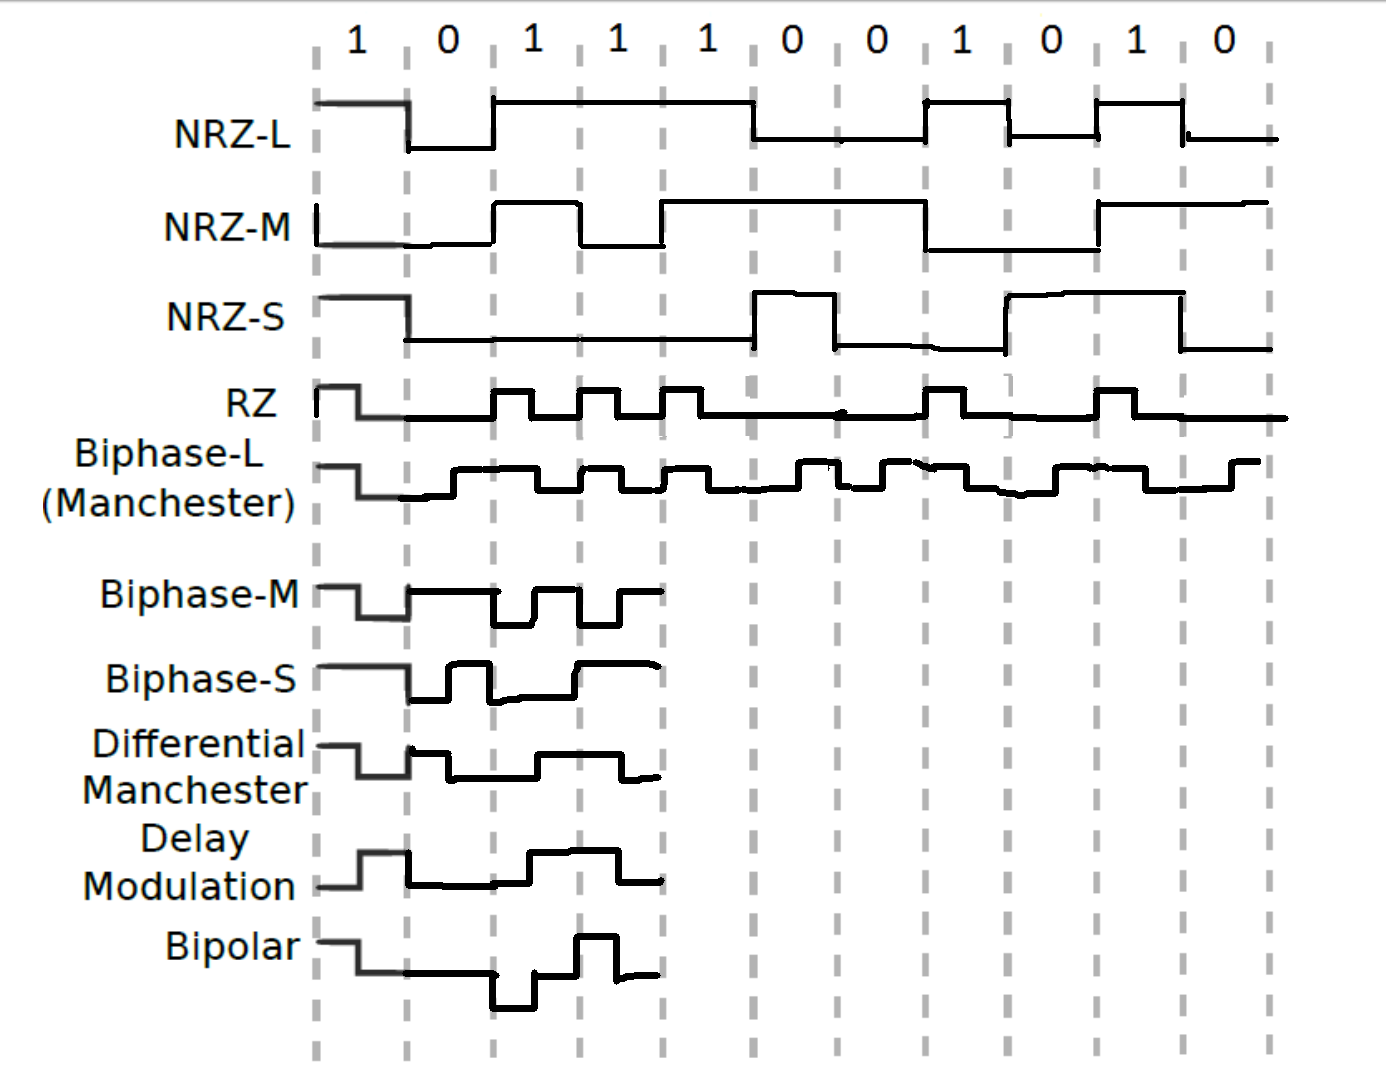
\includegraphics[width=14cm]{Codierungen.png}
\begin{enumerate}
    \item -
    \item Selbsttaktung?
        \begin{itemize}
            \item NRZ-L: Nein, Lange 0er Folge
            \item NRZ-M: Nein, Lange 0er Folge
            \item NRZ-S: Nein, Lange 1er Folge
            \item RZ: Nein, Lange 0er Folge
            \item Biphase-L: Ja
            \item Biphase-M: Ja
            \item Differential Manchester: Ja
            \item Delay Modulation: Ja
            \item Bipolar: Nein, Lange 0er Folge
        \end{itemize}
    \item Minimaler Signalflankenabstand:
        \begin{itemize}
            \item NRZ-L: 10101...
            \item NRZ-M: 10101...
            \item NRZ-S: 10101...
            \item RZ: 11111...
            \item Biphase-L: 00000.... bzw. 11111....
            \item Biphase-M: 11111....
            \item Differential Manchester: 00000...
            \item Delay Modulation: 11111.... bzw. 00000....
            \item Bipolar: 11111...
        \end{itemize}
    \item Selbsttaktende Kodierung mit mindestabstand 3 Zeiteinheiten zwischen Flanken:
        Möglich, man könnte definieren dass 4 aufeinanderfolgende 1er codiert werden
        durch 3 Zeiteinheiten eine 1 und im vierten (und allgemein) Taktung nach Biphase-M.
        4 Aufeinanderfolgende 0er könnte man dementsprechend ähnlich Codieren.
\end{enumerate}



\section*{Aufgabe 2 - Physikalische Übertragungen}
\begin{enumerate}
    \item geschlossene Form der Fourier-Transformation Koeffizienten über dem Intervall $[0;2\pi]$.
        Allgemein: \\
    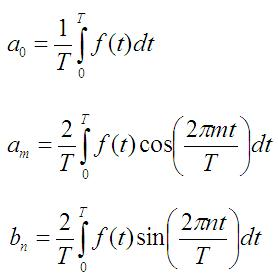
\includegraphics[width=6cm]{optimalcoefficients.jpg} \\
        Hier also ist $a_0 = 1/2$, die ganze cos-reihen fallen weg (da die fkt ungerade ist, f(x) = -f(-x)),
        und die $b_n$'s sind abhängig von n auch entweder $0$ (bei $n$ gerade) oder $2/(\pi * n)$ bei $n$ ungerade. \\ \\
        Die Koeffizienten der gesamten Fourier-Transformation: \\
        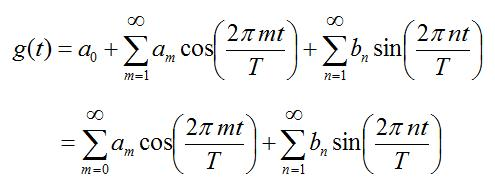
\includegraphics[width=10cm]{fouriersum.jpg} \\
        Und in unserem Fall: $ f(x) = 0.5 + \sum_{n=0}^{\infty}{\frac{-2}{\pi * (2 * n + 1)} * sin((2 * n + 1) * x)} $.
    \item Dämpfung um Faktor 0.3: Wie auch immer die Dämpfung gemeint ist.
    \item $f(x) = 0.5 - \frac{2}{\pi}*sin(x) - \frac{2}{3\pi}*sin(3 x) - \frac{2}{5\pi}*sin(5 x) -
        \frac{2}{7\pi}*sin(7 x) - \frac{2}{9\pi}*sin(9 x) $ \\
        % 0.5 - 2/π sin(x) - 2/(3 π) sin(3 x) - 2/(5 π) sin(5 x) - 2/(7 π) sin(7 x) - 2/(9 π) sin(9 x)
        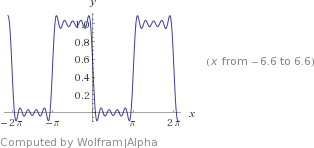
\includegraphics[width=10cm]{graph.png} \\


\end{enumerate}





\end{document}
